% !TeX spellcheck = en_GB
\chapter{Chapter Example}
\label{ch:2chapter}
%------------------------------------------------------
\epigraph{Some very clever idea }{Very clever man \index[cite]{Clever Man}}
%======================================================
\startcontents[chapter]
\printcontents[chapter]{}{-1}{\setcounter{tocdepth}{3}}
\newpage

In this chapter (Chapter~\ref{ch:2chapter}) will be presented unrelated data...I'm really sorry for that.

\section{Molecules}
\label{sec:2ch-molecules}

Please find structures of molecules\footnote{Made in LaTeX as well.} which were used in the study (see Fig.~\ref{fig:molecules}). The data is presented in section \ref{sec:2ch-data} on p.~\pageref{sec:2ch-data}. 
\inputfigure[.5]{Chapter2/molecules}[Studied molecules][molecules][pdf]


\section{Data}
\lettrine[lraise=0.1]{W}{e} discussed earlier that systems studied in this work are photo-activated (\acrshort{RET}, \acrshort{REET}, \acrshort{PET}, Photoisomerization). It simply means that system should be excited from its ground state to some electronic excited state, because only upon being in the excited state the system could be active from the point of displaying useful property. At room temperature thermal energy is not adequate to significantly populate electronically excited states.\par

Here we would like to spent some time to discuss such terms as \emph{state} and the~term~\emph{excited~state}.\par

\begin{wrapfigure}{l}{0.5\linewidth}
	\centering
	\centering
	\addtocounter{totalfigures}{1} 
	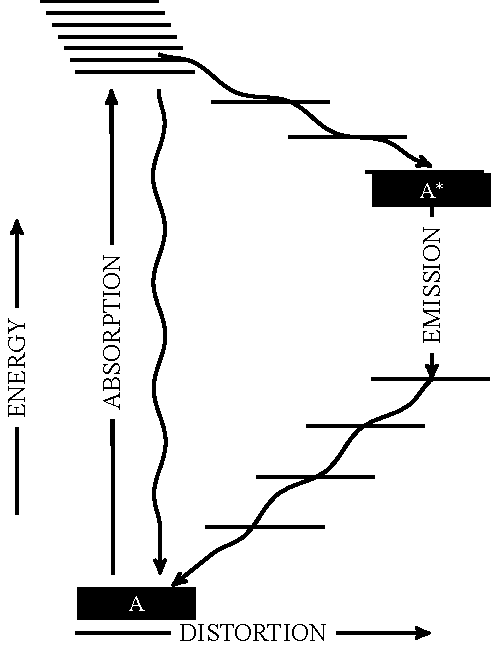
\includegraphics[width=.6\linewidth]{figures/Chapter2/energydistoration}
	\caption{Energy versus distortion diagram\,\cite{adamson-1983}.}
	\label{fig:energydistoration}	
\end{wrapfigure}

The work of Adamson\cite{adamson-1983} we will helpful in the discussion.\par

The word \emph{state} has two different usages in science. To the spectroscopist, the state of a molecule is defined by quantum numbers. He will use term designations and thus speak of the $^2P_{1/2}$ state of the sodium atom or the $^3\Sigma^-_g $ state of $\rm O_2$. In the case of coordination compounds, examples would be the $^4T_{2g}$ and $^2E_g$ ligand field states of Cr(III). When we assign the various absorption maxima in the UV-vis spectrum of a coordination compound, we are proposing specific state-to-state electronic transitions. Thus the first major absorption band for $\rm Cr(NH_3)_6^{3+}$ is assigned as the $^4A_{2g}\rightarrow ^2T_{2g}$ transition. To the spectroscopist, then, an excited state has different electronic (and rotational and vibrational) quantum numbers than does the ground state.\cite{adamson-1983}\par

The word \emph{state} has a rather different meaning in thermodynamics. When we speak of, say, $\rm HCl$ gas at standard conditions, we mean a collection of molecules with a certain average molar energy, entropy, free energy, etc. This is not a single spectroscopic state. Rather, we have a Boltzmann distribution of quantum states. This collection or ensemble has average properties the above thermodynamic ones, and many others, such as density, index of refraction, absorption spectrum, etc. The usual standard state of aqueous $\rm Cr(NH_3)_6^{3+}$ refers to a condition of unit activity under $1$\,atm pressure and at $25^\circ$C. A collection of ions in this state has certain average bond lengths and angles; it has thermodynamic properties; it has chemical reactivity described by one or more rate constants, each having temperature dependence and corresponding activation energy.\cite{adamson-1983}\par

\emph{Excited states} could have different meaning in case of molecular and supramolecular systems. Let take spectroscopic ground state $A$, and a first electronic excited state $ A^*$, illustrated in Figure~\ref{fig:energydistoration}. $ A^*$ will, usually, have different bond lengths and angles than system in state $A$.\par

\begin{wrapfigure}{r}{0.5\linewidth}
	\centering
	\centering
	\addtocounter{totalfigures}{1} 
	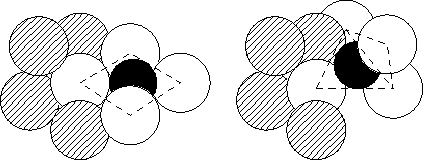
\includegraphics[width=.8\linewidth]{figures/Chapter2/cageeffect}
	\caption{Solvent cage effect in excited state thermal equilibration\,\cite{adamson-1983}.}
	\label{fig:cageeffect}	
\end{wrapfigure}

When light is absorbed by species $A$, a population of $ A^*$ states is produced, and we expect the transition to be a ``vertical" one, that is, electronic rearrangement occurs but no appreciable nuclear motion. Transitions occur in about $10^{-15}$\,s,\footnote{The velocity of an electron making one complete circuit in a Bohr orbit is $\sim 10^{16}$\,\AA/sec. Thus, an electron may move on the order of $10$\,{\AA} in $10^{-15}$\,sec. Since $10$\,{\AA} is the order if size of many commonly encountered groups of atoms (chromophores) responsible for absorption of light, we deduce that the timescales of photon interaction and electron are of the same order of magnitude.\cite{turro-1991}} a time too short for significant displacement of nuclei. The consequence is that $A^*$ molecules are not produced in their equilibrium geometry and should therefore be highly vibrationally excited. This collections of molecules is called Franck-Condon collection or Franck-Condon state ($A^*_{FC}$).\cite{adamson-1983}\par

Assuming that complex $A$ has a square planar geometry, while the equilibrium geometry of $ A^*$ is tetrahedral. A newly formed $A^*$ complex cannot immediately relax to tetrahedral geometry, solvent molecules have to rearrange themselves around (Figure~\ref{fig:cageeffect}); new solvation sphere must be established. As an estimate, it should take roughly about $200$ vibrational periods or about $1$\,ps for a solvent molecule to make diffusional jump from one position to another. The $A^*$ complex is formed in the ground state geometry in a solvent cage that delays its relaxation to the equilibrium geometry. One could expect the collection of molecules $ A^*_{FC}$ to make a succession of configurational adjustments before settling down into an equilibrium Boltzmann distribution of vibrational states. The whole process may take about $10$\,ps. Thermally equilibrated $A^*$ is a thermodynamic state; it represents an ensemble of $A^*$ molecules that is at ambient temperature with respect to vibrations (a solvated molecule really does not have translation or free rotation).\cite{adamson-1983}\par

A representation of molecular electronic state energy levels, with singlet and triplet states in separate columns, is referred to as the Perrin-Jablonski diagram (Figure~~\ref{fig:jablonski-example}). Often, vibrational sublevels are shown schematically as well. Radiative transitions from one level to another are indicated by straight arrows and non-radiative ones by wavy arrows. Most often, the levels correspond to vibrationally relaxed electronic states, \ie to an equilibrium geometry of each individual state. Sometimes, an effort is made to show the state energies at two or more geometries, and as this representation becomes more elaborate, the diagram gradually turns into a drawing of a slice through potential energy surfaces (Figure~\ref{fig:potential-surface}).

\inputfiguresE[1]{Chapter2/Jablonski_cool}{Chapter2/abs-spec}[One possible form of a Perrin-Jablonski diagram, where $I_\pi$ -- ionisation level, $T$ -- triplet and $S$ -- singlet state][The relationship of observed radiative transitions to potential energy curves (schematic)\,\cite{montalti-book-2006}][jablonski-example][potential-surface][.49][.49]


\label{sec:2ch-data}
\inputfigure[1]{Chapter2/RuIandII-emission-77K}[Data for molecules presented on Fig.~\ref{fig:molecules}][RuIandII-emission-77K][pdf]

\begin{equation}
\label{eq:one-level}
\dfrac{dN_1(t)}{dt}=\sigma I(t)-k_1N_1(t)
\end{equation}


Solution of equation~\ref{eq:one-level} is expressed in equation~\ref{eq:solution-one-level}:

\begin{equation}
\label{eq:solution-one-level}
N_1(t)=\dfrac{\sigma \tau_pI_0}{4}\sqrt{\dfrac{\pi}{\ln 2}\exp\left(\dfrac{k_1^2 \tau_p^2}{16\ln2}\right)}\left(1+\erf\left(2\sqrt{\ln 2}\dfrac{t}{\tau_p}-\dfrac{k_1\tau_p}{4\sqrt{\ln2}}\right)\right)\exp(-k_1t)
\end{equation}

To extract deexcitation rate $k_1$ from such function is a complicated mathematical task. Instead of determining $k_1$ as an analytical function, we determined it in an iterative manner, by fitting experimental data as following:

\[
\dfrac{N_{i+1}(t)-N_{i}(t)}{\delta t}=\sigma I(t)-k_1N_i(t),
\]

\noindent so:

\[
N_{i+1}(t)=\left(\sigma I(t)-k_1N_{i}(t)\right)\times \delta t +N_{i}(t),
\] 
\noindent where $\delta t$ is the time step, equalled to $\frac{\text{time-scale}}{N_{points}}$.


\section{Conclusion}
\label{sec:2ch-conslusion}

According to presented data (see Table~\ref{table:Ranges}) we can make conclusions...(see Fig.~\ref{fig:conclusion}).


\inputfigure[1]{Chapter2/PET-Foldamers}[Model for PET in foldamers][conclusion][pdf]



\newpage



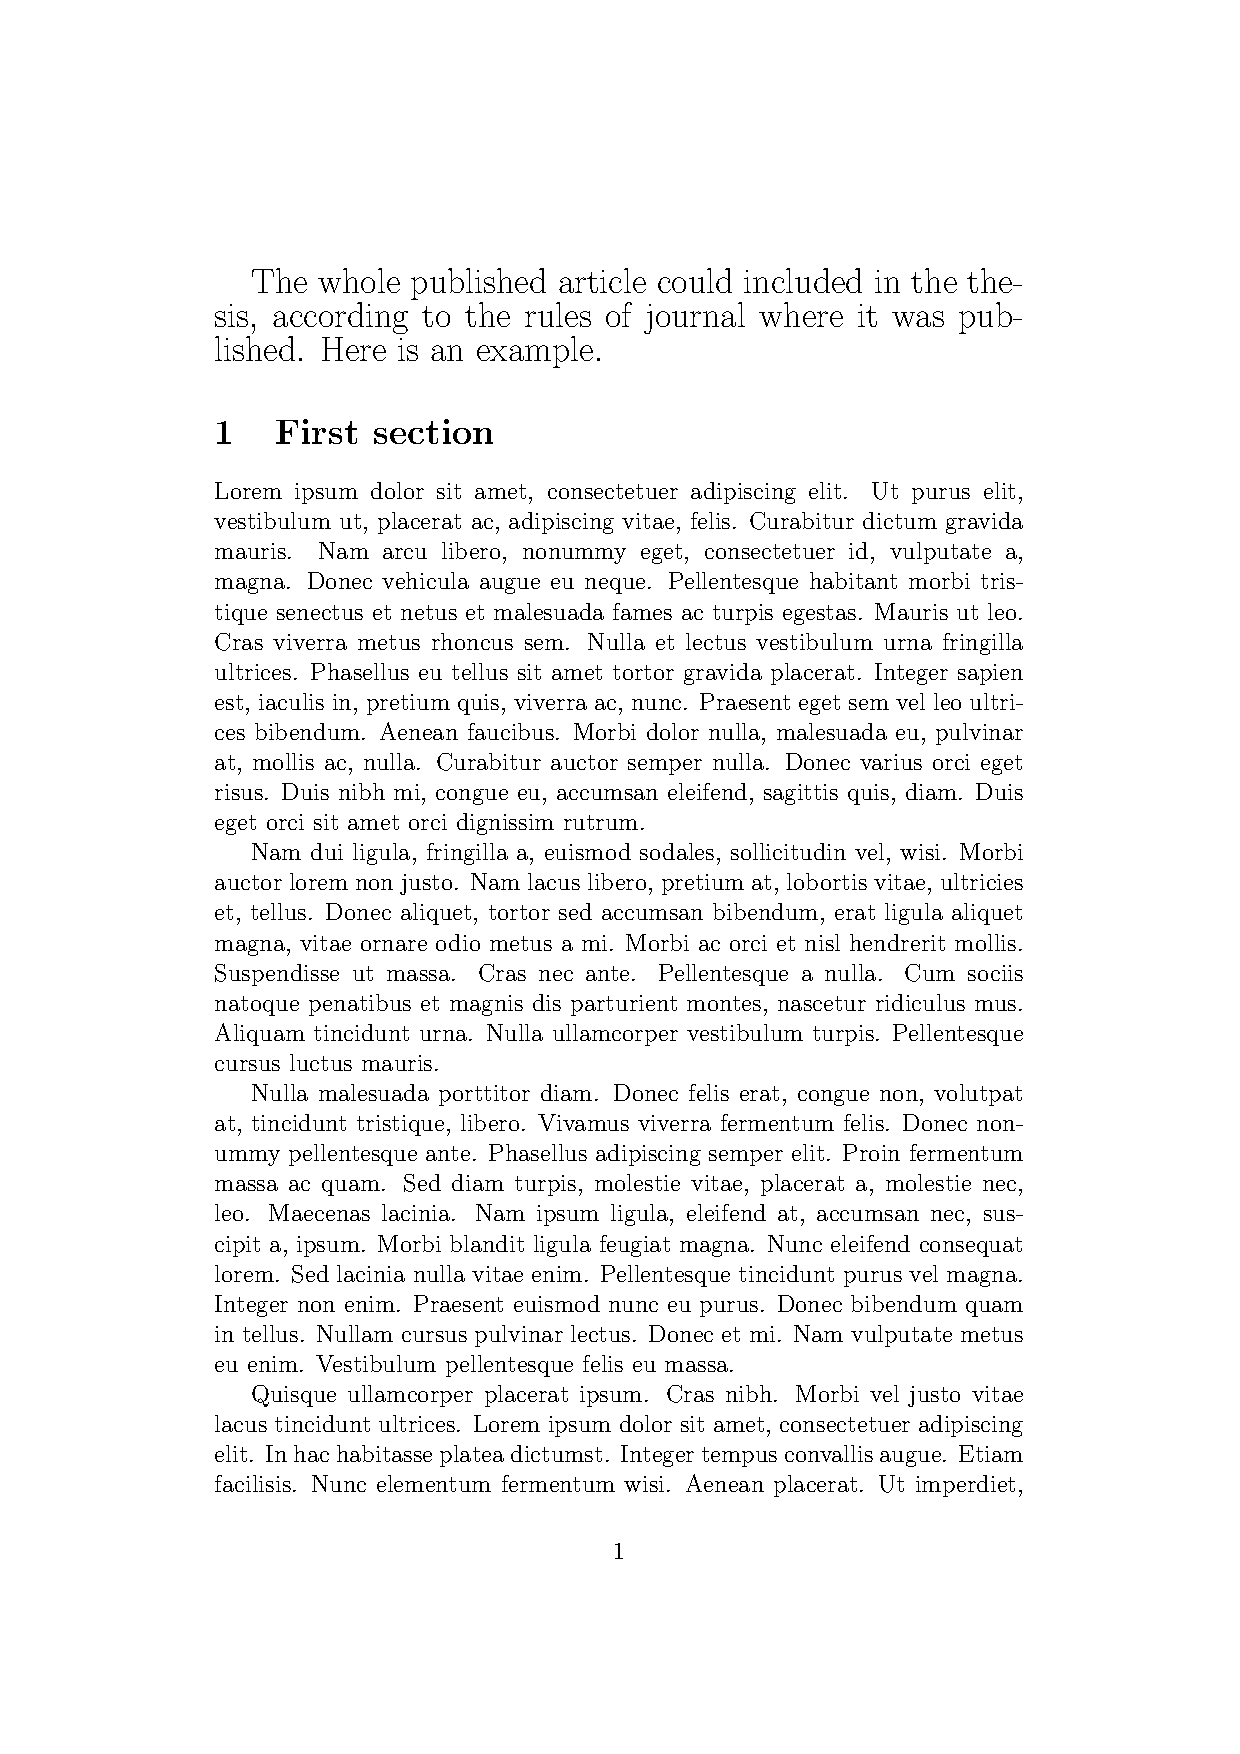
\includepdf[fitpaper=false, pages=-, pagecommand={\thispagestyle{fancy}}, addtotoc={1,section,1,First section, first-sec, 2, section, 1, Second section, sec-sec,2,subsection,2,New subsection,subsec,3,section,1, Third section, third-sec}]{article.pdf}

\stopcontents[chapter]